\documentclass{article}
\usepackage{graphicx}
\begin{document}

\title{CS 3841 Lab 5: Let's Chat}
\author{Jeff Stubler & Matt Edwards}
\date{24 October 2011}
\maketitle

\section*{Introduction}
We started this lab by discussing how we would design and implement it based on the given requirements. It was determined that new threads would be created to handle the UI, keyboard, time ticking, sending messages, receiving messages, and a controller thread to handle all of these. We split the work so Jeff would spend most of his time on the keyboard, time ticking, and sending and receiving of messages, while Matt would work primarily on the UI thread.

\section*{Things that went right and wrong}
Overall, this lab went well but we did not achieve the desired results. In particular, two parts of this lab went well - the server and the UI implementation. Despite this, we were not able to fully implement the lab. Due to the time constraints, being overly ambitious, and unforeseen bugs, we were not able to fully integrate the server to function with the GUI.

\section*{What we learned}
From this lab, we learned that programming sockets in C is a lot more difficult than programming sockets in Java, and protocols that are easy to use with Telnet are easier to develop. Also, we learned how to incorporate the ncurses library to create an elementary GUI with C.

\section*{Time Analysis}
In total Jeff spent about 20 hours working on this and Matt spent about 15. Most of Jeff's time was spent on the server and Matt's was divided among learning how to use ncurses and implementing the UI.

\begin{figure}[!h]
\caption{UI Implementation}
\begin{center}
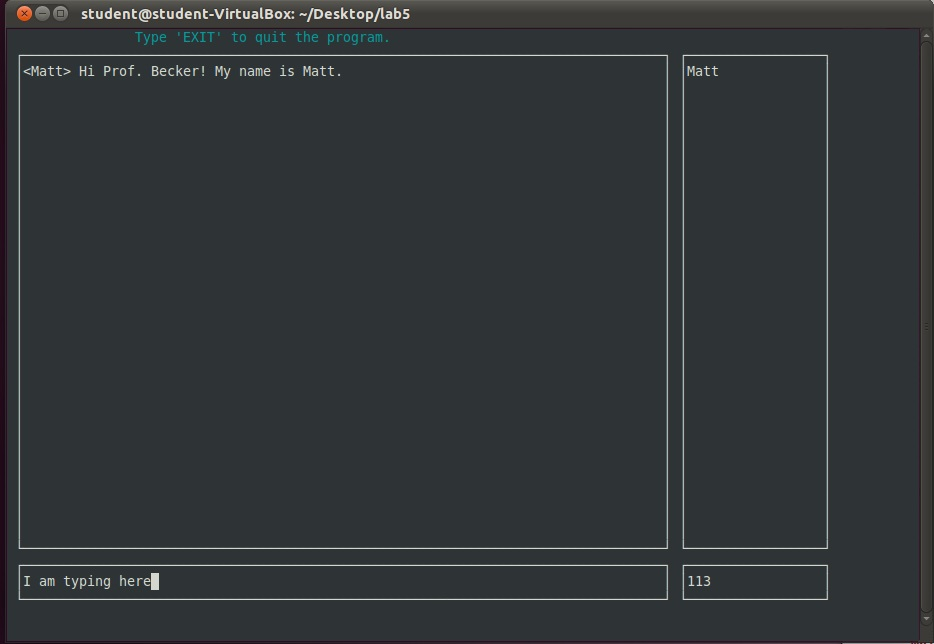
\includegraphics[scale=0.2]{ui.jpg}
\end{center}
\label{UI}
\end{figure}

\section*{Conclusion}
In this lab, we constructed code using POSIX threads, protected against race conditions, communicated using sockets, and implemented a GUI with ncurses. We learned quite a bit from this lab and spent a decent amount of time making trying to implement all desired functionality.

\section*{Appendix: Source code}

\subsection*{controller.c}

\begin{verbatim}


\end{verbatim}

\subsection*{controller.h}

\begin{verbatim}



\end{verbatim}

\subsection*{keyboard.c}

\begin{verbatim}



\end{verbatim}

\subsection*{keyboard.h}

\begin{verbatim}



\end{verbatim}

\subsection*{main.c}

\begin{verbatim}



\end{verbatim}

\subsection*{main.h}

\begin{verbatim}



\end{verbatim}

\subsection*{network.c}

\begin{verbatim}



\end{verbatim}

\subsection*{network.h}

\begin{verbatim}



\end{verbatim}

\subsection*{receive.c}

\begin{verbatim}



\end{verbatim}

\subsection*{receive.h}

\begin{verbatim}



\end{verbatim}

\subsection*{send.c}

\begin{verbatim}



\end{verbatim}

\subsection*{send.h}

\begin{verbatim}



\end{verbatim}

\subsection*{thread.c}

\begin{verbatim}



\end{verbatim}

\subsection*{thread.h}

\begin{verbatim}



\end{verbatim}

\subsection*{tick.c}

\begin{verbatim}



\end{verbatim}

\subsection*{tick.h}

\begin{verbatim}



\end{verbatim}

\subsection*{daemon.c}

\begin{verbatim}



\end{verbatim}

\subsection*{daemon.h}

\begin{verbatim}



\end{verbatim}

\subsection*{main.c}

\begin{verbatim}



\end{verbatim}

\end{document}
